\begin{homeworkProblem}[17][Blood $CO_2$ and Ventilation]
\begin{enumerate}
% Solution 17(a)
\item The old model supposes that the loss of $CO_2$ is only related to
ventilation. However, $CO_2$ can also diffuse spontaneously from high
concentration region to low concentration region. The new model includes this
factor.

% Solution 17(b)
\item The system of equations for $C_n$ and $V_n$ is \begin{align}
    C_{n+1} &= C_{n} - \beta V_nC_n + m\\
    V_{n+1} &= \alpha C_n.
\end{align}
Writing it as a single equation that only depends on $C_n$: \begin{equation}
    C_{n+1} = C_{n} - \alpha\beta C_n C_{n-1} + m \label{eq:CO2_next}
\end{equation}

% Solution 17(c)
\item Suppose $\bar C = C_{n+1} = C_n = C_{n-1}$, substituting $\bar C$ into
\eqref{eq:CO2_next} gives: \[
    \begin{aligned}
    \bar C &= \bar C - \alpha\beta\bar C^2 + m\\
    \bar C^2 &= m/\alpha\beta\\
    \bar C &= \sqrt{m/\alpha\beta} = \bar V/\alpha
    \end{aligned}
\]
To determine whether it's stable or not, we need to make the absolute value of
the roots of the characteristic function smaller than 1: \[
    \lambda^2 - b \lambda + c = 0
\]
where \[
    \begin{aligned}
        b &= \left.\pderiv{f}{C}\right|_{\bar C, \bar V} +
        \left.\pderiv{g}{V}\right|_{\bar C, \bar V} \\
        c &= \left.\pderiv{f}{C}\right|_{\bar C, \bar V}
        \left.\pderiv{g}{V}\right|_{\bar C, \bar V} -
        \left.\pderiv{f}{V}\right|_{\bar C, \bar V}
        \left.\pderiv{g}{C}\right|_{\bar C, \bar V}
    \end{aligned}
\]
Here \[
    \begin{aligned}
        f(C, V) &= C - \beta CV + m\\
        g(C, V) &= \alpha C
    \end{aligned}
\]
So \[
    \begin{aligned}
        b &= (1- \beta \bar V) = 1 - \sqrt{\alpha\beta m}\\
        c &= -\alpha(-\beta \bar C) = \sqrt{\alpha\beta m}
    \end{aligned}
\]
Recall that we derived in the book that if both eigenvalues have magnitude less
than 1, then \[
    \left\{
    \begin{aligned}
        &2 > 1 + c > |b|, & b^2 - 4c > 0\\
        &1 > c > |b/2|^2, & b^2 - 4c < 0
    \end{aligned}
    \right.
\]
Either way, when $c = \sqrt{\alpha\beta m} < 1$, both inequities hold. So
if we want the steady state to be stable, we need to have \[
    m\alpha \beta < 1
\]

% Solution 17(d)
\item We can have oscillation when the characteristic equation has complex
eigenvalues. To make this happen, we need to have \[
    b^2 - 4c = (1 - \sqrt{m\alpha\beta})^2 - 4\sqrt{m\alpha\beta} < 0
\]
Substitute $x = \sqrt{m\alpha\beta}$, then we should have \[
    x^2 - 6x + 1 < 0
\]
Solving this inequity gives \[
    3 - 2\sqrt{2} < x < 3+2\sqrt{2}
\]i.e., when we have$|x-3| < 2\sqrt{2}$, where $x = \sqrt{m\alpha\beta}$, there
will be oscillation in $V_n$ and $C_n$.

% Solution 17(e)
\item The system of equations will look like \begin{align}
    C_{n+1} &= C_n - \beta V_nC_n + m \label{eq:new_CO2_next}\\
    V_{n+1} &= \frac{V_{\max}C^\mathcal{l}_n}{K^{\mathcal{l}}+C^\mathcal{l}_{n}}
    \label{eq:new_ventilation_next}
\end{align}
It's trivial to show that if we write \eqref{eq:new_ventilation_next} as
\begin{equation}
    V_{n} = \frac{
        V_{\max}C^\mathcal{l}_{n-1}}{K^{\mathcal{l}}+C^\mathcal{l}_{n-1}}
    \label{eq:new_ventilation}
\end{equation}
and plug \eqref{eq:new_ventilation} to \eqref{eq:new_CO2_next}, then we'll have
\begin{equation}
    C_{n+1} = C_n - \beta \frac{
        V_{\max}C^\mathcal{l}_{n-1}C_n}{K^{\mathcal{l}}+C^\mathcal{l}_{n-1}}
        + m
\end{equation}

% Solution 17(f)
\item The relationship between $\mathcal{S}(C)$ and $\mathcal{l}$ is shown in
Figure \ref{fig:CO2_sensitivity}. $K$ is chosen to be $50$.
\begin{SCfigure}[8][h]
    \centering
    \caption[The relationship between $\mathcal{S}(C)$ and $\mathcal{l}$]{
        The relationship between $\mathcal{S}(C)$ and $\mathcal{l}$.
    }
    \label{fig:CO2_sensitivity}
    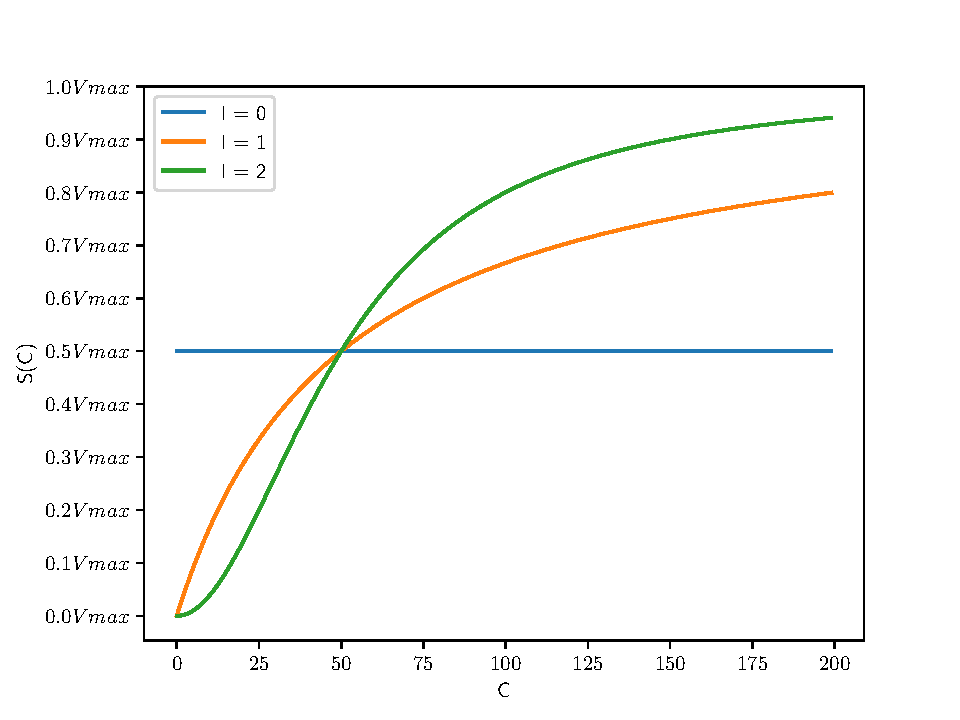
\includegraphics[scale=0.6]{fig/fig17(f).pdf}
\end{SCfigure}

% Solution 17(g)
\item For steady state of $C_n$ and $V_n$, we have \begin{equation}
        \bar C = \bar C - \beta \frac{V_{\max} \bar C^{\mathcal{l}+1}}{
        K^{\mathcal{l}} + \bar C^\mathcal{l}} + m \label{eq:stable_power}
\end{equation}
Rearrange \eqref{eq:stable_power} we can derive the following equation 
\eqref{eq:17gsol}, which is what the question wanted
\begin{equation}
    \boxed{\frac{m}{\beta} = \frac{V_{\max} \bar C^{\mathcal{l}+1}}{
            K^{\mathcal{l}} + \bar C^\mathcal{l}} = \bar C \bar V}
    \label{eq:17gsol}
\end{equation}

\pagebreak

% Solution 17(h)
\item When $\mathcal{l} = 1$, \[\begin{aligned}
    C_{n+1} &= C_n - \beta V_nC_n + m\\
    V_{n+1} &= \frac{V_{\max}C_n}{K+C_{n}}
\end{aligned}\]
and \begin{equation}
    C_{n+1} = C_n - \beta \frac{V_{\max}C_{n-1}C_n}{K+C_{n-1}}+ m
    \label{eq:stable}
\end{equation}
Suppose $\bar C = C_{n+1} = C_n = C_{n-1}$ and plug it into \eqref{eq:stable},
\begin{align}
    &\bar C - \beta \frac{V_{\max}\bar C^2}{K + \bar C} + m = \bar C\\
    &\frac{\bar C^2}{K + \bar C} = \frac{m}{\beta V_{\max}} \label{eq:sub}\\
    &\bar C^2-\frac{m}{\beta V_{\max}}\bar C - \frac{m}{\beta V_{\max}}K = 0
\end{align}
Let $\delta = \frac{m}{\beta V_{\max}}$, then \[
    \begin{aligned}
        \bar C &= \frac{1}{2}\left(\delta \pm \sqrt{\delta^2+4K\delta}\right)\\
        \bar V &= \frac{V_{\max} \bar C}{K + \bar C}
    \end{aligned}
\]
We need to make the roots for the characteristic equation have a magnitude $< 1$
again:
\[
    \lambda^2 - b\lambda + c = 0
\]
where \[
    \begin{aligned}
        b &= \left.\pderiv{f}{C}\right|_{\bar C, \bar V} +
        \left.\pderiv{g}{V}\right|_{\bar C, \bar V} \\
        c &= \left.\pderiv{f}{C}\right|_{\bar C, \bar V}
        \left.\pderiv{g}{V}\right|_{\bar C, \bar V} -
        \left.\pderiv{f}{V}\right|_{\bar C, \bar V}
        \left.\pderiv{g}{C}\right|_{\bar C, \bar V}
    \end{aligned}
\]
Here \[
    \begin{aligned}
        f(C, V) &= C - \beta CV + m\\
        g(C, V) &= \frac{V_{\max}C}{K+C}
    \end{aligned}
\]
So
\begin{align}
    b &= (1- \beta \bar V) = 1- \frac{\beta V_{\max}\bar C}{K+\bar C}
    \label{eq:b}\\
    c &= \frac{\beta  V_{\max} K \bar C}{(K + \bar C)^2}\label{eq:c}
\end{align}
Use \eqref{eq:sub} to make \eqref{eq:b} and \eqref{eq:c} look prettier:
\[
    \begin{aligned}
        b &= 1 - \frac{m}{\bar C}\\
        c &= \frac{m^2K}{\beta V_{\max} \bar C^3}
    \end{aligned}
\]
Recall again that we derived in the book that if both eigenvalues have magnitude
less than 1, then \[
    2 > 1 + c > |b|
\]
Therefore we should have \[
    \frac{m^2K}{\beta V_{\max} \bar C^3} < 1
\]
Note that if $\bar C = \delta - \sqrt{\delta^2 + 4K\delta}$, it will be $< 0$
since $\delta^2 + 4K\delta > \delta^2$, which will make the inequity trivially 
true (it's not biologically meaningful anyway since negative blood $CO_2$ 
concentration seems deadly). So the inequity will become \[
    \frac{m^2K}{\beta V_{\max}} < \bar C^3 = 
    \left( \frac{m}{\beta V_{\max}} + 
    \sqrt{\left(\frac{m}{\beta V_{\max}}\right)^2 + 
    \frac{4Km}{\beta V_{\max}}}\right)^3
\]
(It looks a bit difficult to simplify for me. So I'll leave it be.)

% Solution 17(i)
\item If we want oscillation to happen, then the characteristic equation should 
have complex roots, i.e.: \[
    b^2 - 4c = \left(1 - \frac{m}{\bar C}\right)^2 - 
    \frac{4m^2K}{\beta V_{\max}\bar C^3} < 0
\]

Consider $l > 1$, with $\pderiv{f}{C}$, $\pderiv{f}{V}$ and $\pderiv{g}{V}$ 
unchanged, we'll have \[
    \begin{aligned}
    \pderiv{g}{C} &= 
    \frac{
        \mathcal{l} V_{\max} C^{\mathcal{l} - 1}(K^\mathcal{l} + C^\mathcal{l})
        - \mathcal{l}V_{\max} C^{\mathcal{l}} C^{\mathcal{l} - 1}}{
            (K^{\mathcal{l}} + C^{\mathcal{l}})^2
        }\\
    &= \frac{\mathcal{l} V_{\max} K^{\mathcal{l}}C^{\mathcal{l}-1}}{
        (K^{\mathcal{l}} + C^{\mathcal{l}})^2
    }
    \end{aligned}
\]
This will make \[
    c = \frac{\mathcal{l} \beta V_{\max} K^{\mathcal{l}}\bar C^{\mathcal{l}}}{
        (K^{\mathcal{l}} + \bar C^{\mathcal{l}})^2
    }
\]
For oscillation to happen, we still need to have \[
    b^2 - 4c < 0
\]
\end{enumerate}

\end{homeworkProblem}